\documentclass[11pt]{template}

\member{1}{Noemi Bongiorni}{noemibongiorni}{278173}
\member{2}{Alessandro Pedone}{alepedone}{273814}
\member{3}{Simone Licciardi}{simonegabolalicc}{214875}
\member{4}{Federico Maria Riva}{rfeder}{280447}

\teamname{NoPainNoTrain}

\begin{document}

\head

\begin{multicols}{2}

       
\section{Introduction} Mars terrain segmentation is a key part of the process that precedes human exploration of the planet allowing to detect potential landing zone and areas of interest. This project aims to segment gray scale images of Mars terrain among five disjoint classes (\emph{Background [0], Soil [1], Bedrock [2], Sand [3], Big Rock [4]}) through one or more UNet.

\section{Problem Analysis}
To assess the task, we perform a visual inspection of the dataset, determining its relevant characteristics and noticing several outliers.

\textbf{Dataset inspection.}
The dataset consists of a \texttt{(2615, 2, 64, 128)} tensor, that contains 2615 images and 2615 corresponding labels/masks, both with \texttt{(64x128)} as spatial dimensions.

\textbf{Main challenges.}
Visual inspection reveals the main learning challenges.
\begin{itemize}
    \item There are 110 images (4.2\%) where a \textit{superimposed alien} is present, as shown in \ref{fig:filters1}. Despite the fact that the aliens are placed in different ways and are difficult to detect directly, we exploit the fact that the corresponding masks, shown in \ref{fig:filters2}, are all the same. This allows us to remove all these images from the dataset, resulting in a clean \texttt{(2505, 2, 64, 128)} tensor.
    \item There is an \emph{unbalanced} distribution of samples among the classes. In particular, the background is predominant, and to address this problem, we could utilize different techniques, such as class weights and the inclusion of dice loss. Class [4], on the other hand, is significantly underrepresented compared to the others, an issue that could be addressed using the image blending technique.
    \item The segmentation, at first glance, seems a bit \textit{coarse}, which could be managed by applying geometric transformations to the images and using boundary-sensitive loss functions, such as focal loss and boundary loss.
\end{itemize}


\begin{figure}[H]
        \begin{subfigure}{\linewidth}
            \centering
            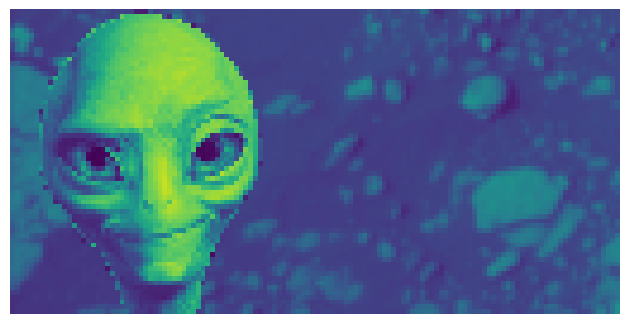
\includegraphics[width=0.75\linewidth]{assets/alien_image.png}
            \caption{Example of a image of an alien}
            \label{fig:filters1}
        \end{subfigure}
        \begin{subfigure}{\linewidth}
            \centering
            
\includegraphics[width=0.75\linewidth]{assets/alien_label.png}
            \caption{The mask common to all images of aliens}
            \label{fig:filters2}
        \end{subfigure}
\end{figure}

\textbf{Initial assumptions.}
We assume that for each image there is no ambiguity on its unique mask (equivalently, that either the model is correct, or is mistaken), that all mistakes weight the same towards our downstream tasks, that the images have no preferred orientation and that zoom is constant.
                
\section{Method}
To develop our solution, we split the filtered dataset into test (10\%) and train\_validation (90\%) sets. We further divided the latter in validation (10\%) and train (90\%). 
We fine-tune hyperparameters, such as the number of \textbf{epochs, batch size, learning rate} (including strategies like learning rate warm-up), and \textbf{patience} levels for early stopping.
In order to mitigate overfitting, we use \textbf{early stopping, regularization, data augmentation} and weight initialization to ensure stable convergence.
Moreover while studying early-stopping we tried to monitor mean\_iou metric instead of accuracy in order to prove a better feedback to the training without getting any improvement due to oscillations.
Additionally, we incorporate class weights and pixel distribution (class weight refinement) to address the imbalance between classes.
In order to extrapolate more information from a single image, we increment the number of channels using the following \textbf{computer vision methods} (implemented with custom layers): thresholding, edge detection, laplacian, wavelet.
We design a \textbf{simple architecture} that we can consider a baseline, emphasizes interpretability and allows us to test the effectiveness of some of the already mentioned techniques.
All the consideration are made on small simple UNet composed by two \textbf{UNet blocks} for both the down-sampling and up sampling paths. Each single UNet blocks is made of a Conv2D, Batchnormalization and Activation layers. 
At the beginning, we try to implement a \textbf{dual UNet model} via two identical UNets (same depths and UNet block). Then we move to two different nets in order to capture both local and global details of the image (Global and Local Nets).
In order to combine the two outputs given by the subnets we consider different techniques: concatenation, addition, continuation and addition and fusion mechanism. 
Our \textbf{loss function} is based on a combination of sparse categorical cross-entropy (ignoring background), focal loss, dice loss, a loss limiting the number of classes predicted to 2 (termed \textit{class limit loss}) and a boundary loss. We also test a low-pass filter loss to encourage uniform transitions in classes predicted. The latter 2 losses are due to domain knowledge information: we observe that maps usually contain only a few classes (rarely more than 2) and that the transition between classes happened in a rather continuous and uniform manner. Some loss weights are established before-hand by setting their weight as fixed, while other were chosen with a dynamical rule based on accuracy and mean\_iou metrics. We choose starting and fixed weights by inspecting graphically the model's predictions against ground truth, and choosing the type of error to compensate.
We focus on \textbf{data augmentation} too, with the scope of enhancing model robustness. We try to utilize standard geometric transformations (flip, translation, zoom), because the others results in a clear drop in performance due to excessive distortion of the images, but we aren't able to pull off in an effective set of transformation and it turn out to be irrelevant or counterproductive in terms of performance. We also choose to implement \textbf{images and masks blending} with successful results.
Due to training instabilities, Adam's and AdamW's noisy behavior and lack of plateau, we investigate \textbf{optimizers} with better convergence properties. We test Lion with a Reduce on Plateau callback, AdamW with warm-up and Cosine Decay and AdamW with Warm-Restart Cosine Decay. The first frequently get caught in non-desirable minima, the second achieves results similar to those of AdamW, the last doesn't improve substantially on the second. So we settled for \texit{AdamW with Cosine Decay} and Early Stopping callback. 

\section{Experiments}
As summarized in Table \ref{tab:1} (Where the performances of the most relevant networks for the development of our neural network are reported), we add complexity to the network, conducting a series of experiments by progressively modifying the baseline UNet architecture to assess the impact of each change on model performance.

\begin{center}
\centering
\setlength{\tabcolsep}{3pt}
\captionof{table}{performance of all our experiments.}
\begin{tabularx}{.5\textwidth}{lYcY}
    \toprule
    Model & Test Set mean IoU & Kaggle mean IoU\\
    \midrule
    Baseline  & 32.81 & 32.459\\
    Network 1 & 23.89 & 37.051\\
    Network 2 & 42.68 & 44.082\\
    Network 3 & 39.9 & 46.326\\
    Network 4 & 66.6 & 39.675\\
    Network 5 & 47.0 & 46.967\\
    Network 6 & 42.86 & 48.459\\
    Network 7 & 49.08 & 48.267\\
    Network 8 & 49.04 & 50.731\\
    Network 9 & 62.99 & 61.984\\
    Network 10 & 50.43 & 49.736\\
    Final Model & 61.76 & 64.910\\
    \arrayrulecolor{black}\bottomrule
\end{tabularx}
\label{tab:1}
\end{center}
\begin{description}[leftmargin=!]
  \item[\textbf{Baseline Network}] was a standard UNet (2 downsampling, 2 upsampling blocks, 128-sized bottleneck) trained on the complete dataset (2118 images).
  
  \item[\textbf{Network 1}] improves on \textbf{Baseline Network} by training the model on the dataset filtered as described above. This improves model performance, leveraging better-quality data.
  
  \item[\textbf{Network 2}] improves on \textbf{Baseline Network} by adding channels that filter information about the image; particularly, we added thresholding, edge detection, laplacian and wavelet filters. They were added in an incremental fashion (that is, one by one, by monitoring performance). This improves model performance, leveraging better information extraction.
  
  \item[\textbf{Network 3}] improves on \textbf{Network 1} and \textbf{Network 2} with an optimizer that weights classes differently based on their frequency (computed on pixel distribution). This guarantees that Mode Collapse doesn't happen.
  
  \item[\textbf{Network 4}] tried to improve on \textbf{Network 2} by adding a geometric augmentation pipeline, as mentioned above, rather than adding channels. It failed on performance metrics and was abandoned.
  
  \item[\textbf{Network 5}] improves on \textbf{Network 3} by implementing a learning rate warm-up and Cosine Decay schedule to the AdamW optimizer. Together with this, we also tested SGD, Lion with Reduce on Plateau, and learning rate Warm-Restarts.
  
  \item[\textbf{Network 6}] adapts the architecture from \textbf{Network 3} and implements a Dual UNet architecture.
  
  \item[\textbf{Network 7}] implements adaptive normalization. It failed on performance metrics and was abandoned.
  
  \item[\textbf{Network 8}] improves on \textbf{Network 6} by making the two parallel UNet architectures differ: one tries to implement a global point of view over the data, the other one acts locally. Bottleneck-wise, the former uses a size of 512, storing richer information, while the latter uses 128. To combine the output, we empirically established that concatenation works best.
  
  \item[\textbf{Network 9}] integrates the learning rate schedule from \textbf{Network 5}, by adding losses based on domain knowledge and weights established either by hyperparameter sweep (class limit loss) or an adaptive procedure (cross-entropy, focal, dice loss). We also tested a low-pass metric without performance improvement.

  \item[\textbf{Network 10}] implements inside the \textbf{Network 9} architecture the Squeeze-Excitation block and dilated convolutions. We tried making the training longer, but if failed on performance metrics and was abandoned.
  
  \item[\textbf{Final Model}] improves on \textbf{Network 9} by adding He weights and image/mask blending.
\end{description}
% We observed that the vast majority of segmentations comprised pixels from just 1 or 2 classes. Therefore, we introduced a loss penalizing predictions that exceeded the 2-class limit, in an effort to push down the number of predicted classes for each image. We added this regularization term to the objective function, with w

\section{Results}
The \textbf{final model} we submitted on Kaggle scored $64.910\%$. Overall, the improvement on the baseline is significant.
\section{Discussion}
\textit{Strengths}: loss function choice, feature extraction with computer vision methods, data augmentation tailored to the situation, effective optimization, model complexity. 
\textit{Weakness}: a beneficial modification can worsen other aspects and an intervention that has a positive impact on one network doesn’t always have the same effect on another. 
\textit{Limitation}: the coarse segmentation of the training set might have caused the model to learn biases or miss important patterns. Despite this, visually, the predicted masks seemed more accurate than those in the dataset.

\section{Conclusions}
Future areas of development include refining data augmentation, using GANs, enhancing encoders with pretrained models, optimizing bottlenecks, and exploring new architectures, including detective networks, but also leveraging more scientific literature.
\nocite{*}
\bibliographystyle{abbrv}
\bibliography{ref}

\end{multicols}
\end{document}